%%%%%%%%%%%%%%%%%%%%%%%%%%%%%%%%%%%%%%%%%%%%%%%%%%%%%%%%%%%%%%%%%%%%%%%%%%%%
% AGUJournalTemplate.tex: this template file is for articles formatted with LaTeX
%
% This file includes commands and instructions
% given in the order necessary to produce a final output that will
% satisfy AGU requirements, including customized APA reference formatting.
%
% You may copy this file and give it your
% article name, and enter your text.
%
%
% Step 1: Set the \documentclass
%
%

%% To submit your paper: 
\documentclass[draft]{agujournal2019}
\usepackage{url} %this package should fix any errors with URLs in refs.
\usepackage{lineno} 
\usepackage[inline]{trackchanges} %for better track changes. finalnew option will compile document with changes incorporated.
\usepackage{soul}
\usepackage{graphicx}
\graphicspath{{../bounce_figures/important/}}
\linenumbers
%%%%%%%
% As of 2018 we recommend use of the TrackChanges package to mark revisions.
% The trackchanges package adds five new LaTeX commands:
%  
%  \note[editor]{The note}
%  \annote[editor]{Text to annotate}{The note}
%  \add[editor]{Text to add}
%  \remove[editor]{Text to remove}
%  \change[editor]{Text to remove}{Text to add}
%
% complete documentation is here: http://trackchanges.sourceforge.net/
%%%%%%%

\draftfalse

%% Enter journal name below.
%% Choose from this list of Journals:
%
% JGR: Atmospheres
% JGR: Biogeosciences
% JGR: Earth Surface
% JGR: Oceans
% JGR: Planets
% JGR: Solid Earth
% JGR: Space Physics
% Global Biogeochemical Cycles
% Geophysical Research Letters
% Paleoceanography and Paleoclimatology
% Radio Science
% Reviews of Geophysics
% Tectonics
% Space Weather
% Water Resources Research
% Geochemistry, Geophysics, Geosystems
% Journal of Advances in Modeling Earth Systems (JAMES)
% Earth's Future
% Earth and Space Science
% Geohealth
%
% ie, \journalname{Water Resources Research}

\journalname{Enter journal name here}


\begin{document}



\title{Scale Sizes of Bouncing Microbursts}

%% ------------------------------------------------------------------------ %%
%
%  AUTHORS AND AFFILIATIONS
%
%% ------------------------------------------------------------------------ %%

% Authors are individuals who have significantly contributed to the
% research and preparation of the article. Group authors are allowed, if
% each author in the group is separately identified in an appendix.)

% List authors by first name or initial followed by last name and
% separated by commas. Use \affil{} to number affiliations, and
% \thanks{} for author notes.
% Additional author notes should be indicated with \thanks{} (for
% example, for current addresses).

% Example: \authors{A. B. Author\affil{1}\thanks{Current address, Antartica}, B. C. Author\affil{2,3}, and D. E.
% Author\affil{3,4}\thanks{Also funded by Monsanto.}}

\authors{Wyatt Wetzel\affil{1}, John Sample\affil{1}}


% \affiliation{1}{First Affiliation}
% \affiliation{2}{Second Affiliation}
% \affiliation{3}{Third Affiliation}
% \affiliation{4}{Fourth Affiliation}

\affiliation{1}{Montana State University}
%(repeat as many times as is necessary)

%% Corresponding Author:
% Corresponding author mailing address and e-mail address:

% (include name and email addresses of the corresponding author.  More
% than one corresponding author is allowed in this LaTeX file and for
% publication; but only one corresponding author is allowed in our
% editorial system.)

% Example: \correspondingauthor{First and Last Name}{email@address.edu}

% \correspondingauthor{=name=}{=email address=}

%% Keypoints, final entry on title page.

%  List up to three key points (at least one is required)
%  Key Points summarize the main points and conclusions of the article
%  Each must be 140 characters or fewer with no special characters or punctuation and must be complete sentences

% Example:
% \begin{keypoints}
% \item	List up to three key points (at least one is required)
% \item	Key Points summarize the main points and conclusions of the article
% \item	Each must be 140 characters or fewer with no special characters or punctuation and must be complete sentences
% \end{keypoints}

% \begin{keypoints}
% \item enter point 1 here
% \item enter point 2 here
% \item enter point 3 here
% \end{keypoints}

%% ------------------------------------------------------------------------ %%
%
%  ABSTRACT and PLAIN LANGUAGE SUMMARY
%
% A good Abstract will begin with a short description of the problem
% being addressed, briefly describe the new data or analyses, then
% briefly states the main conclusion(s) and how they are supported and
% uncertainties.

% The Plain Language Summary should be written for a broad audience,
% including journalists and the science-interested public, that will not have 
% a background in your field.
%
% A Plain Language Summary is required in GRL, JGR: Planets, JGR: Biogeosciences,
% JGR: Oceans, G-Cubed, Reviews of Geophysics, and JAMES.
% see http://sharingscience.agu.org/creating-plain-language-summary/)
%
%% ------------------------------------------------------------------------ %%

%% \begin{abstract} starts the second page

\begin{abstract}
(passive vs active?)
We present a collection of bouncing microbursts observed by the HILT instrument on SAMPEX from 1994-2004.
The statistical properties of these microbursts are analyzed, and an estimate of their scale sizes are obtained. 
We find that that the majority of bouncing microbursts observed by SAMPEX have scale sizes on the order of $10^2km$. 
\end{abstract}

% \section*{Plain Language Summary}
% [ enter your Plain Language Summary here or delete this section]





\section{Introduction}
Radiation belt electron populations are determined by a variety of source and loss processes. 
An important loss process is pitch angle scattering of electrons by plasma waves, which depletes the radiation belts by losing electrons to the atmosphere. 
Whistler mode chorus waves in particular scatter electrons into microbursts, which are short ($<100$ms) increases in precipitating electron flux. 

Microbursts were first observed in the form of Bremsstrahlung x-rays by balloon borne detectors \cite{balloon_burst_first} in year.
Modleing has shown that microbursts are potentially an important loss process, capable of emptying the radiation belts on the order of a day \cite{micro_loss} (what does this actually mean)
An important parameter in determining the importance of microbursts as a loss process is their scale size. 
Estimates from various papers
 

Microbursts are sometimes observed in trains that descend in amplitude.
These are known as ``bouncing microbursts'' as they appear to be the same packet of electrons being observed multiple times as they bounce between their mirror points \cite{Blake96}. 
They are characterized in time series data by several microbursts separated by one bounce period, each decreasing in amplitude as more electrons are lost to the atmosphere on each bounce.
The time between each microburst could also be half a bounce period, if two microbursts are generated from the same event and are launched northward and southward.  

Bouncing microbursts offer a unique opportunity to measure properties of the microburst. 
Repeated observations of the same microburst allow us to estimate the particle's scale size, and do other things i suppose
Bouncing microbursts have been observed by SAMPEX \cite{Blake96} and the FIREBIRD-II cubesats \cite{fire_bounce}, from which estimates of the scale size of the microbursts were obtained. 

A collection of bouncing microbursts would be useful to estimate a distribution of scale sizes for microbursts as a whole, rather than a scattering of estimates from individual microbursts.




\begin{figure}
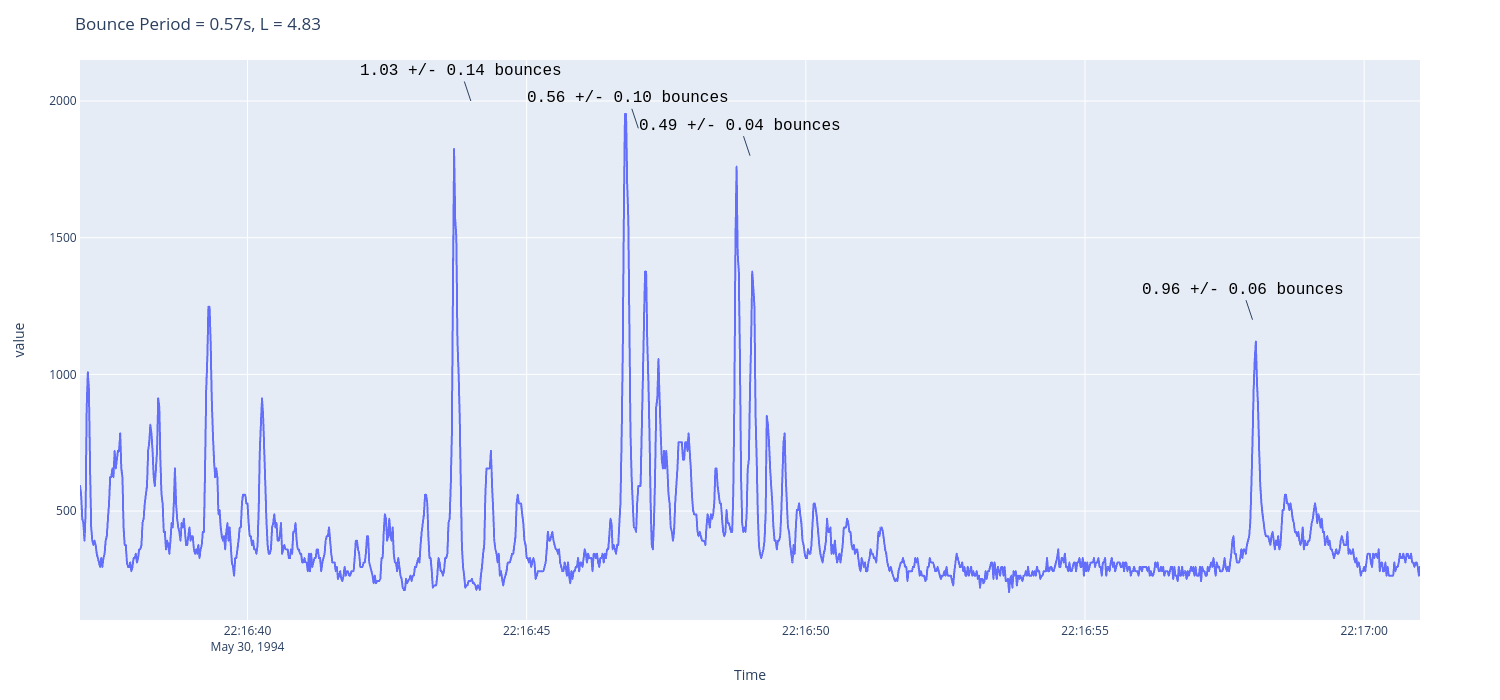
\includegraphics[width=\textwidth]{case_study.png}
\caption{A series of bouncing microbursts in succession. The time between peaks is labeled in units of the bounce period for $1$MeV electrons. }
\end{figure}

 
\section{Bouncing Microburst Algorithm}
To search for bouncing microbursts in the $20$ms SAMPEX data, we construct a correlation based algorithm. %bad
We construct several ``kernels'', which are artificial data designed to look like bouncing microbursts. 
These kernels are constructed of Gaussians with various separations ranging from $.05$s to $1$s to attempt to capture bouncing microbursts with a variety of bounce periods. 
We then take the cross correlation of the SAMPEX time series data and each of the kernels, and flag places with high correlation for manual review. 
We also require that each flagged location contain a microburst as defined by the O'Brien parameter \cite{obrien_parameter}. 

The algorithm initially identified 7107 candidates, which were narrowed down to 892 bouncing microbursts by hand. 
Improvements could be made to the algorithm, as it has an extremely high false positive rate. 

\section{Location}
With this collection of bonucing microbursts, the statistical properties of these events can be studied. 
The majority of these events occur in two bands, between L shells $2$ and $4$, with a smaller population at $L>6$. 
The occurrence characteristics of microbursts in SAMPEX data have been studied \cite{burst_occurrence} and microbursts are most frequent between $L=4$ and $L=6$; however, the bouncing microbursts found in this study are least likely to occur in this band. 
This discrepancy could be cause by the sheer number of microbursts making it difficult to pick out bouncing microbursts; any unrelated microburst occuring in the middle of an observation of a bouincing microburst will mean that bouncing microburst will be rejected, possibly artificially deflating the frequency of observations in the band where microbursts are most likely to occur. 
Most bouncing microbursts in this study occur in the morning sector between $0$ and $12$ magnetic local time, which aligns with the occurrence characteristics of microbursts in general as found by \citeA{burst_occurrence}.

\begin{figure}[h!]
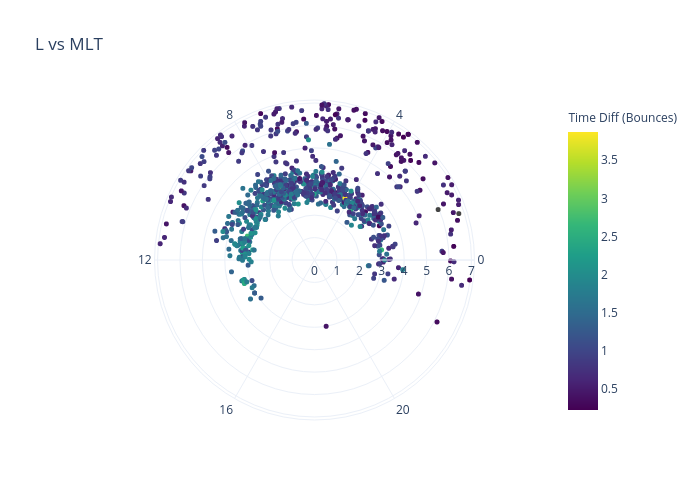
\includegraphics[width=\textwidth]{dial.png}
\caption{Locations of bouncing microbursts in L and MLT. Color scale indicates average distance between peaks in units of the bounce period of $1$MeV electrons at the edge of the loss cone.  }
\end{figure}

\section{Bounce Period Distribution}
One may expect that the time between peaks in a bouncing microburst would be one bounce period, or half of a bounce period if two microbursts are launched from their source region moving in opposite directions. 
However, the distribution of time differences between peaks in units of bounce periods has peaks not at $.5$ and $1$, but at approximately $.7$ and $1.7$ as shown in Fig. \ref{fig:periods}

\begin{figure}[h!]
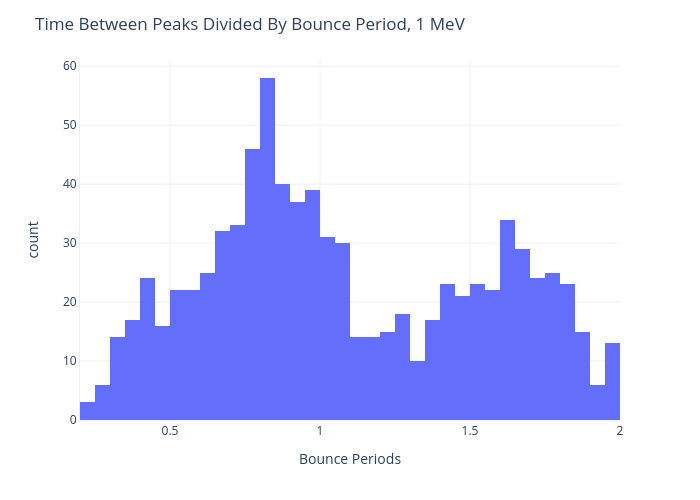
\includegraphics[width=.5\textwidth]{period_hist_1_MeV.png}
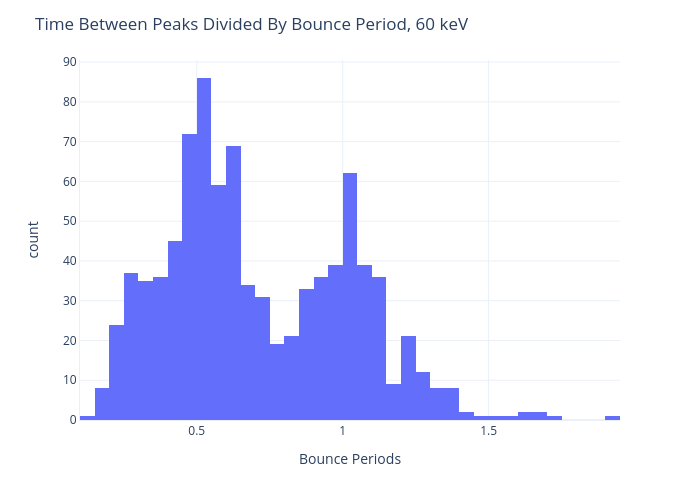
\includegraphics[width=.5\textwidth]{period_hist_60_keV.png}
\label{fig:periods}
\caption{Distribution of time between peaks measured in bounce periods. Fig a) shows the distribution calculated for 1MeV electrons mirroring at 100km, and fig b) shows the distribution calculated for 60 keV electrons mirroring at 30deg mlat.}
\end{figure} 

Thus far we have assumed that each peak in a bonucing microburst corresponds to the same microburst bouncing between mirror points, or to two microbursts generated in the same region simultaneously.
The data however suggest that a substantial number of the collected events are not made of microbursts generated from a single event.

Whistler mode chorus often occur in groups of short discrete elements. 
There are several parameters used to characterize whistler mode chorus, including their repetition rate \cite{repetition_rate}.  
Microbursts are often associated with chorus waves, and repetitive wave-particle interaction between chorus and electrons (at the equator?) could produce ``bouncing'' microbursts with time scales defined by the chorus repetition rate and not the bounce period of the electrons in the microburst. 

\cite{repetition_rate} studied whistler mode chorus waves in $L>5$ and their repetition rates. 

**********
how to compare my data with theirs? most samples are $L<5$ 
******
\section{Scale Sizes}
Measurements of bouncing microbursts allow us to compute the local scale size of the microburst, and from that the equatorial scale size. 
The loacl scale size of each microburst is computed as 

\begin{equation}
 l_{obs} = T v_D  = T \frac{2 \pi}{\tau_D} (1+ \frac{A}{R_e}) \cos \lambda 
\end{equation}
where $T$ is the time between the first and last bounce observed, $v_D$ is the drift velocity of electrons at magnetic latitude $\lambda$, $A$ is the altitude of SAMPEX at the observation, $R_e$ is the radius of the Earth, and $\tau_D= (60)(62.7)(\frac{MeV}{E})(\frac{1}{L})s$ is the drift period of an electron at an energy $E$ and L-shell $L$. 
\begin{figure}[h!]
 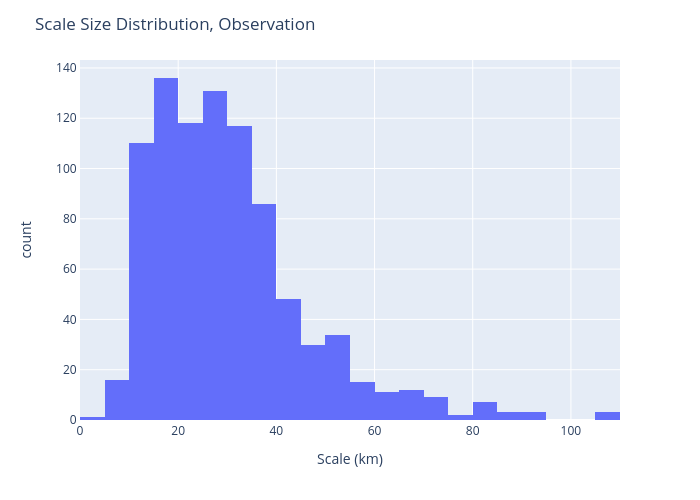
\includegraphics[width=\textwidth]{scale_hist_local.png}
 \label{fig:local}
 \caption{Local scale size, calculated at SAMPEX's location at time of observation.}
\end{figure}
The resulting distribution of local scale sizes of the microbursts we have collected is presented in \ref{fig:local}.

We can convert the scale size at the location of the observation to the microburst's size at the equator with Gauss' law, setting the flux at SAMPEX's location equal to the flux at the equator:

\begin{equation}
 B_{eq} l_{eq}^2 = B_{obs} l_{obs}^2
\end{equation}
where $B_{eq}$ and $B_{obs}$ are the magnitudes of the magnetic field at the equator and at SAMPEX, and $l_{eq}$ and $l_{obs}$ are the scale sizes of the microburst at the equator and at SAMPEX.

Idealizing Earth's magnetic field as a dipole, we find that the equatorial scale size of the microbursts is 

\begin{equation}
l_{eq} = l_{obs} \sqrt{2} \left( \frac{L R_e}{r_{obs} } \right)^{3/2}
\end{equation}

where $r_{obs}$ is the distance from the center of the Earth to the location of the observation.

\begin{figure}[h!]
 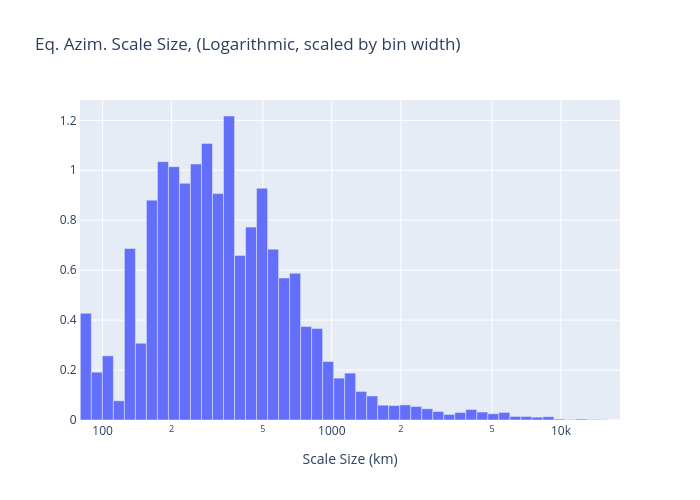
\includegraphics[width=\textwidth]{log_eq_scales.png}
 \caption{Equatorial azimuthal scale sizes, binned on a logarithmic scale and weighted by bin width.}
 \label{fig:log_eq_scales}
\end{figure}

\section{Conclusions}
***

should have comparison to other papers with estimations of scale size - Mike's FIREBIRD paper, blake 96, others?

what does scale size tell us specifcally about microbursts? size of generation region? 

***

The microbusrts studied here have scale sizes mostly on the order of $10^2$km.
Previous stud(ies?) have found bouncing microbursts with equatorial scale sizes of $530$km \cite{fire_bounce}, others?.
\cite{Blake96} observed that the relative infrequency of bouncing microbursts compared to solitary bursts indicates that most microbursts must have scale sizes of less than a few tens of kilometers, which was the minimum size of microburst that SAMPEX could observe bouncing. 
The bouncing microbursts in this paper therefore represent the population of larger microbursts, not microbursts as a whole.
It can be seen in Fig. \ref{fig:log_eq_scales} that the frequency of bouncing microbursts drops off substantially at lower scale sizes, which is as we would expect as SMAPEX is less able to observe bouncing microbursts of smaller scales. 

These scale sizes are similar to the scale sizes of whistler mode chorus waves \cite{chorus_scales}, the primary candidate for the waves that generate microbursts.
%Text here ===>>> 

%%

%  Numbered lines in equations:
%  To add line numbers to lines in equations,
%  \begin{linenomath*}
%  \begin{equation}
%  \end{equation}
%  \end{linenomath*}



%% Enter Figures and Tables near as possible to where they are first mentioned:
%
% DO NOT USE \psfrag or \subfigure commands.
%
% Figure captions go below the figure.
% Table titles go above tables;  other caption information
%  should be placed in last line of the table, using
% \multicolumn2l{$^a$ This is a table note.}
%
%----------------
% EXAMPLE FIGURES
%
% \begin{figure}
% \includegraphics{example.png}
% \caption{caption}
% \end{figure}
%
% Giving latex a width will help it to scale the figure properly. A simple trick is to use \textwidth. Try this if large figures run off the side of the page.
% \begin{figure}
% \noindent\includegraphics[width=\textwidth]{anothersample.png}
%\caption{caption}
%\label{pngfiguresample}
%\end{figure}
%
%
% If you get an error about an unknown bounding box, try specifying the width and height of the figure with the natwidth and natheight options. This is common when trying to add a PDF figure without pdflatex.
% \begin{figure}
% \noindent\includegraphics[natwidth=800px,natheight=600px]{samplefigure.pdf}
%\caption{caption}
%\label{pdffiguresample}
%\end{figure}
%
%
% PDFLatex does not seem to be able to process EPS figures. You may want to try the epstopdf package.
%

%
% ---------------
% EXAMPLE TABLE
% Please do NOT include vertical lines in tables
% if the paper is accepted, Wiley will replace vertical lines with white space
% the CLS file modifies table padding and vertical lines may not display well
%
%  \begin{table}
%  \caption{Time of the Transition Between Phase 1 and Phase 2$^{a}$}
%  \center
%  To add line numbers to lines in equations:
%  \begin{linenomath*}
%  \begin{equation}
%  \end{equation}
%  \end{linenomath*}
% 
% 
%  \begin{tabular}{l c}
%  \hline
%   Run  & Time (min)  \\
%  \hline
%    $l1$  & 260   \\
%    $l2$  & 300   \\
%    $l3$  & 340   \\
%    $h1$  & 270   \\
%    $h2$  & 250   \\
%    $h3$  & 380   \\
%    $r1$  & 370   \\
%    $r2$  & 390   \\
%  \hline
%  \multicolumn{2}{l}{$^{a}$Footnote text here.}
%  \end{tabular}
%  \end{table}

%% SIDEWAYS FIGURE and TABLE
% AGU prefers the use of {sidewaystable} over {landscapetable} as it causes fewer problems.
%
% \begin{sidewaysfigure}
% \includegraphics[width=20pc]{figsamp}
% \caption{caption here}
% \label{newfig}
% \end{sidewaysfigure}
%
%  \begin{sidewaystable}
%  \caption{Caption here}
% \label{tab:signif_gap_clos}
%  \begin{tabular}{ccc}
% one&two&three\\
% four&five&six
%  \end{tabular}
%  \end{sidewaystable}

%% If using numbered lines, please surround equations with \begin{linenomath*}...\end{linenomath*}
%\begin{linenomath*}
%\begin{equation}
%y|{f} \sim g(m, \sigma),
%\end{equation}
%\end{linenomath*}

%%% End of body of article

%%%%%%%%%%%%%%%%%%%%%%%%%%%%%%%%
%% Optional Appendix goes here
%
% The \appendix command resets counters and redefines section heads
%
% After typing \appendix
%
%\section{Here Is Appendix Title}
% will show
% A: Here Is Appendix Title
%
%\appendix
%\section{Here is a sample appendix}

%%%%%%%%%%%%%%%%%%%%%%%%%%%%%%%%%%%%%%%%%%%%%%%%%%%%%%%%%%%%%%%%
%
% Optional Glossary, Notation or Acronym section goes here:
%
%%%%%%%%%%%%%%
% Glossary is only allowed in Reviews of Geophysics
%  \begin{glossary}
%  \term{Term}
%   Term Definition here
%  \term{Term}
%   Term Definition here
%  \term{Term}
%   Term Definition here
%  \end{glossary}

%
%%%%%%%%%%%%%%
% Acronyms
%   \begin{acronyms}
%   \acro{Acronym}
%   Definition here
%   \acro{EMOS}
%   Ensemble model output statistics
%   \acro{ECMWF}
%   Centre for Medium-Range Weather Forecasts
%   \end{acronyms}

%
%%%%%%%%%%%%%%
% Notation
%   \begin{notation}
%   \notation{$a+b$} Notation Definition here
%   \notation{$e=mc^2$}
%   Equation in German-born physicist Albert Einstein's theory of special
%  relativity that showed that the increased relativistic mass ($m$) of a
%  body comes from the energy of motion of the body—that is, its kinetic
%  energy ($E$)—divided by the speed of light squared ($c^2$).
%   \end{notation}

% 
% \newpage
% \section{Open Research}
% AGU requires an Availability Statement for the underlying data needed to understand, evaluate, and build upon the reported research at the time of peer review and publication.
% 
% Authors should include an Availability Statement for the software that has a significant impact on the research. Details and templates are in the Availability Statement section of the Data and Software for Authors Guidance: \url{https://www.agu.org/Publish-with-AGU/Publish/Author-Resources/Data-and-Software-for-Authors#availability}
% 
% It is important to cite individual datasets in this section and, and they must be included in your bibliography. Please use the type field in your bibtex file to specify the type of data cited. Options include [Dataset], [Software], [ComputationalNotebook], [Collection].
%Example:
%
%@misc{https://doi.org/10.7283/633e-1497,
%  doi = {10.7283/633E-1497},
%  url = {https://www.unavco.org/data/doi/10.7283/633E-1497},
%  author = {de Zeeuw-van Dalfsen, Elske and Sleeman, Reinoud},
%  title = {KNMI Dutch Antilles GPS Network - SAB1-St_Johns_Saba_NA P.S.},
%  publisher = {UNAVCO, Inc.},
%  year = {2019},
%  type = {dataset}
%}


% For physical samples, use the IGSN persistent identifier, see the International Geo Sample Numbers section:
% \url{https://www.agu.org/Publish-with-AGU/Publish/Author-Resources/Data-and-Software-for-Authors#IGSN}
%%%%%%%%%%%%%%%%%%%%%%%%%%%%%%%%%%%%%%%%%%%%%%%

% \acknowledgments
% This section is optional. Include any Acknowledgments here.
% The acknowledgments should list:\\
% All funding sources related to this work from all authors\\
% Any real or perceived financial conflicts of interests for any author\\
% Other affiliations for any author \newline that may be perceived as having a conflict of interest with respect to the results of this paper.\\
% \clearpage
% It is also the appropriate place to thank colleagues and other contributors. AGU does not normally allow dedications.\\
%\input{methods}
% Hello here is some text in Nick's file
%\input{data}


%% ------------------------------------------------------------------------ %%
%% References and Citations

%%%%%%%%%%%%%%%%%%%%%%%%%%%%%%%%%%%%%%%%%%%%%%%
%
\bibliography{/home/wyatt/LatexFiles/master}
%
% don't specify bibliographystyle

% In the References section, cite the data/software described in the Availability Statement (this includes primary and processed data used for your research). For details on data/software citation as well as examples, see the Data & Software Citation section of the Data & Software for Authors guidance
% https://www.agu.org/Publish-with-AGU/Publish/Author-Resources/Data-and-Software-for-Authors#citation

%%%%%%%%%%%%%%%%%%%%%%%%%%%%%%%%%%%%%%%%%%%%%%%

% \bibliography{}



%Reference citation instructions and examples:
%
% Please use ONLY \cite and \citeA for reference citations.
% \cite for parenthetical references
% ...as shown in recent studies (Simpson et al., 2019)
% \citeA for in-text citations
% ...Simpson et al. (2019) have shown...
%
%
%...as shown by \citeA{jskilby}.
%...as shown by \citeA{lewin76}, \citeA{carson86}, \citeA{bartoldy02}, and \citeA{rinaldi03}.
%...has been shown \cite{jskilbye}.
%...has been shown \cite{lewin76,carson86,bartoldy02,rinaldi03}.
%... \cite <i.e.>[]{lewin76,carson86,bartoldy02,rinaldi03}.
%...has been shown by \cite <e.g.,>[and others]{lewin76}.
%
% apacite uses < > for prenotes and [ ] for postnotes
% DO NOT use other cite commands (e.g., \citet, \citep, \citeyear, \citealp, etc.).
% \nocite is okay to use to add references from your Supporting Information
%



\end{document}



% More Information and Advice:

%% ------------------------------------------------------------------------ %%
%
%  SECTION HEADS
%
%% ------------------------------------------------------------------------ %%

% Capitalize the first letter of each word (except for
% prepositions, conjunctions, and articles that are
% three or fewer letters).

% AGU follows standard outline style; therefore, there cannot be a section 1 without
% a section 2, or a section 2.3.1 without a section 2.3.2.
% Please make sure your section numbers are balanced.
% ---------------
% Level 1 head
%
% Use the \section{} command to identify level 1 heads;
% type the appropriate head wording between the curly
% brackets, as shown below.
%
%An example:
%\section{Level 1 Head: Introduction}
%
% ---------------
% Level 2 head
%
% Use the \subsection{} command to identify level 2 heads.
%An example:
%\subsection{Level 2 Head}
%
% ---------------
% Level 3 head
%
% Use the \subsubsection{} command to identify level 3 heads
%An example:
%\subsubsection{Level 3 Head}
%
%---------------
% Level 4 head
%
% Use the \subsubsubsection{} command to identify level 3 heads
% An example:
%\subsubsubsection{Level 4 Head} An example.
%
%% ------------------------------------------------------------------------ %%
%
%  IN-TEXT LISTS
%
%% ------------------------------------------------------------------------ %%
%
% Do not use bulleted lists; enumerated lists are okay.
% \begin{enumerate}
% \item
% \item
% \item
% \end{enumerate}
%
%% ------------------------------------------------------------------------ %%
%
%  EQUATIONS
%
%% ------------------------------------------------------------------------ %%

% Single-line equations are centered.
% Equation arrays will appear left-aligned.

% Math coded inside display math mode \[ ...\]
%  will not be numbered, e.g.,:
%  \[ x^2=y^2 + z^2\]
% 
%  Math coded inside \begin{equation} and \end{equation} will
%  be automatically numbered, e.g.,:
%  \begin{equation}
%  x^2=y^2 + z^2
%  \end{equation}
% 
% 
% To create multiline equations, use the
% \begin{eqnarray} and \end{eqnarray} environment
% as demonstrated below.
% \begin{eqnarray}
%   x_{1} & = & (x - x_{0}) \cos \Theta \nonumber \\
%         && + (y - y_{0}) \sin \Theta  \nonumber \\
%   y_{1} & = & -(x - x_{0}) \sin \Theta \nonumber \\
%         && + (y - y_{0}) \cos \Theta.
% \end{eqnarray}
% 
%If you don't want an equation number, use the star form:
%\begin{eqnarray*}...\end{eqnarray*}

% Break each line at a sign of operation
% (+, -, etc.) if possible, with the sign of operation
% on the new line.

% Indent second and subsequent lines to align with
% the first character following the equal sign on the
% first line.

% Use an \hspace{} command to insert horizontal space
% into your equation if necessary. Place an appropriate
% unit of measure between the curly braces, e.g.
% \hspace{1in}; you may have to experiment to achieve
% the correct amount of space.


%% ------------------------------------------------------------------------ %%
%
%  EQUATION NUMBERING: COUNTER
%
%% ------------------------------------------------------------------------ %%

% You may change equation numbering by resetting
% the equation counter or by explicitly numbering
% an equation.

% To explicitly number an equation, type \eqnum{}
% (with the desired number between the brackets)
% after the \begin{equation} or \begin{eqnarray}
% command.  The \eqnum{} command will affect only
% the equation it appears with; LaTeX will number
% any equations appearing later in the manuscript
% according to the equation counter.
%

% If you have a multiline equation that needs only
% one equation number, use a \nonumber command in
% front of the double backslashes (\\) as shown in
% the multiline equation above.

% If you are using line numbers, remember to surround
% equations with \begin{linenomath*}...\end{linenomath*}

%  To add line numbers to lines in equations:
%  \begin{linenomath*}
%  \begin{equation}
%  \end{equation}
%  \end{linenomath*}



